\section{DUNE Computing Model}
\label{sec:computing_model}

\subsection{Introduction}
The main purpose of the Computing Model is to guide the creation of DUNE computing fabric, spanning
hardware, middleware and various software components. Such fabric would give to all members of the DUNE
and to raw data for calibration and any other activities as required by the scientific objectives of the experiment.
To meet these goals, and in fulfillment of the data access requirements (\ref{sec:rules-of-access-to-data})
the model presented here is based on distributed data management and Grid and Cloud Computing concepts.

As stated in \ref{sec:modelrole}, the Computing Model is built on the basis of two supporting documents: the
``Software and Computing Requirements'', which sets forth policies and practices for the DUNE computing sector
(Section\,\ref{sec:requirements}), and ``DUNE Data Characteristics'' (Section\,\ref{sec:data-characteristics}) which contains information
necessary for quantifying parameters of the Computing Model. Both documents will be referenced extensively in this section.

Unless stated, no final technology choices are made in this section -- due to a long period of time before the DUNE commissioning,
this will need to be done at a later date and in compliance with the ``Requirements''. Where appropriate, existing systems are described and
considered for use in DUNE.

\subsection{Data rate and volume estimates}
\label{sec:data-rate-and-volume-estimates}
\subsubsection{Overview}
Rate and volume of the various data to be produced in DUNE are perhaps the main driver determining the parameters
of the Computing Model. Data rates for different types and their relationships were considered in Section~\ref{sec:data-characteristics},
and the material below will present a summary and aggregated estimates for the scale of the data of various types
and origin.

It is important to keep in mind that estimates presented in Section~\ref{sec:data-characteristics} were developed under ``baseline''
assumptions necessary for groundwork done in the process of developing the DUNE Conceptual Design Report (CDR).
As DUNE is engaged in R\&D aimed at optimal design of the detector and the physics tools, it is likely that these assumptions will be
revisited at some point and the data rate and volume estimates will need to be revised correspondingly.

\subsubsection{Raw Data}
Characteristics of the data to be produced by DUNE detector systems have been considered in
Sec.~\ref{sec:data-characteristics}.

At the time of writing estimations for the Far Detector data are better understood when compared to other DUNE subsystems,
due to better developed geometry and parameters of the LArTPC, technology and configuration choices, and considerations
presented in subsections~\ref{sec:daq-assumptions} (notes on DAQ),~\ref{sec:zs-data} (Zero Suppression) and \ref{sec:data-compression} (Compression).

A distinguishing characteristic of the data flow in DUNE Far Detector is a significant data reduction factor to be achieved
in the Far Detector DAQ, as evidenced by the numbers presented in Tables~\ref{tab:full-stream-volume} and \ref{tab:zs-volume}.
The key assumption in this is the capability of DAQ to distinguish low energy signals  due to $^{39}$Ar decays spread
across the volume of the detector from more interesting physics phenomena (see~\ref{sec:ar39decays}).
This and similar capabilities will be provided
by deploying appropriate algorithms on the DAQ RCE and online farm utilizing about a hundred computers (estimated).
Estimates of volume of data due to high-energy interaction (cosmic $\mu$ and beam neutrinos) are presented in
Table~\ref{tab:fd-data-volume-summary} (page \pageref{tab:fd-data-volume-summary}) and are quite modest.

Processing required to identify candidate SNB and nucleon decay events will also be handled by the DAQ system and its online farm.
As discussed in subsection \ref{sec:snb-data}, once a SNB trigger condition has been established, the data must
be recorded without zero suppression in order to capture the characteristically low energy and scattered ionization
clusters in the detector volume as expected in a supernova burst event. As shown in Table~\ref{tab:zs-volume} (page~\pageref{tab:zs-volume}),
the resulting volume of data is significant and is currently estimated as just over half a PB annually, given the premise of accepting roughly
12 false positives per year (at this point a benchmark number used solely to set the scale of the data, as commented in~\ref{sec:snb-data}).

Identifying candidate nucleon decay events will also require algorithms that would set the trigger condition consistent
with signatures such as $p \rightarrow K^+\nu$. As shown in \ref{sec:pdk-data}, the volume of data due to such candidate
events is not expected to be appreciable compared to other sources.

The Near Detector is quite different from the Far Detector in all of its characteristics, and it includes a number of subdetectors
such as Fine-Grained Tracker, Electromagnetic Calorimeter and others (see~\ref{sec:nds-event-rates}). There are a few technology
options being conisdered and most parameters are still being finalized at the time of writing, so data estimates are very preliminary.
It is
%conservatively
assumed that the annual volume of these data will be 100\,TB.

%Current numbers result in annual volume from a few dozen to a hundred TB.

%In summary, it is anticipated that under assumptions presented above the total volume of data in DUNE to be
%committed to storage will be up to 1PB per year of data taking.

\subsubsection{Monte Carlo Data}
As discussed in \ref{sec:mc-data-estimates}, the Far and Near Detector simulation is the top contributor to the volume of overall
Monte Carlo in DUNE, with combined annual output of about 35\,TB of data. Other MC data sources are not appreciable.
It is reasonable to expect that this number will grow as more effort becomes available for Monte Carlo studies and
as they become more sophisicated. However, at the time of writing there is no reliable estimate of how this segment of data
will scale over the years.


\subsubsection{Summary of Annual Data Volume Estimates}
\label{summary-annual-volume}
Table~\ref{tab:summary-data-table} contains a summary of estimations for various sources
of data in DUNE, in terms of projected annual volume, which is based on information developed in
this document up to this point. Where applicable, entries are marked with ZS (Zero-Suppression) or
FS (Full-Stream). Atmospheric $\nu$ were not included as discussed in \ref{sec:atmo-nu}. Solar $\nu$ were not
included either, although for a different reason (see~\ref{sec:solar-data}).
\begin{table}[ht!]
	\centering
	\begin{tabular}{| p{1.2in}| p{1.73in} | p{1.5in} | p{0.62in} |}
		\hline
		\textbf{Data Type} & \textbf{Source} & \textbf{ZS/FS} & \textbf{Volume} \\ \hline
		Raw & cosmic-$\mu$  & ZS$^*$ \textit{(see comments)}& 4.8\,TB \\	\hline
		Raw & beam-$\nu$  & ZS$^*$ \textit{(see comments)}& 5.3\,GB  \\	\hline
		Raw & Nucleon Decay Cand.  & ZS$^*$ \textit{(see comments)}& 480\,GB  \\	\hline
		Raw & SNB Cand. (12\,year$^{-1}$) & FS & 553\,TB \\	\hline \hline % \hline
		Raw & Near Detector & ZS & 100\,TB \\	\hline \hline \hline
		Raw & \textbf{Total Raw} & - & \textbf{658\,TB} \\		\hline \hline \hline
		MC & Beamline and Target  & - & 1\,TB \\	\hline
		MC & Far Detector & ZS$^{**}$  \textit{(see comments)}  & 15\,TB \\		\hline
		MC & Near Detector & - &20\,TB \\ \hline \hline \hline
		MC & \textbf{Total MC} & - & \textbf{36\,TB} \\		\hline \hline \hline
		Derived &  Raw  & - & 5.2\,PB \\	\hline
		Derived &  MC  & - & 288\,TB \\	\hline  \hline \hline
		Derived & \textbf{Total Derived} & - & \textbf{5.8\,PB} \\		\hline \hline \hline
		All & \textbf{Grand Total} & - & \textbf{6.5\,PB} \\		\hline % \hline \hline
	\end{tabular}
	\caption{Summary of annual data volume estimates due to various sources.}
	\label{tab:summary-data-table}
\end{table}
Comments to the table:
\begin{itemize}
\item ($^*$) Estimates for the raw data ($\nu$ and $\mu$ but not Supernova canidates) assume ``smart'' Zero Suppression, i.e. extended
window around the peak of the pulse where data is preserved regardless of its instantaneous value (see \ref{sec:zs-data} on page~\pageref{sec:zs-data})

\item ($^{**}$) As discussed in~\ref{sec:data-compression}, at present the zero-suppression algorithms employed in production of the
MC data are not very efficient, so there is potential for further data reduction

\item Entries for the Derived Data -- ESD/AOD --  include the multiplicative ``headroom factor'' of 4 (see justification in \ref{sec:derived-data})
on top of extrapolated factor of 2 which is approximate ratio of the volume of derived data to raw data (\ref{sec:derived-data-factor}).
\end{itemize}

\subsubsection{Implications of the Estimates and Possible Optimization of Data Collection Parameters}
\label{sec:implications-of-data-estimates}
The items summarized in Table~\ref{tab:summary-data-table} have been prepared under a set of specific
assumptions as documented in corresponding subsections of Section~\ref{sec:data-characteristics}.

Even without revisiting much detail, salient features the data volume distribution across various sources are
obvious. The SNB data are the largest source of data by a large margin. This is due to a combination of factors such as:
\begin{itemize}

\item The requirement that SNB candidate data in general should not be discarded (see justification in \ref{sec:snb-data}).

\item The requirement of high sensitivity of DUNE to the Supernova Burst candidate events, which provides motivation
for the trigger logic to be set at high sensitivity (hence the declared number of expected false positives, which is nominal
and is mainly included to set the scale).

\item The requirement that the SNB candidate events are recorded essentially without Zero-Suppression to ensure that low energy
clusters of ionization spread in the detector volume are captured with proper efficiency.

\item The requirement that the digitized data is being read out from the Far Detector LArTPC and recorded continuously over
the nominal window of 10\,s (longer recording periods may in fact be desirable).

\item Large total number of channels in the Far Detector (over 1.5\,million).

\end{itemize}

\noindent
It is also obvious from Table~\ref{tab:summary-data-table} that the very events that constitute the main science objective of DUNE
out of a few -- the beam-$\nu$ events -- produce a tiny nominal amount of data when compared to other sources. From the standpoint
of resource utilization, this may or may not be optimal and further guidance will be needed from the Collaboration.

It may become helpful then to consider adjustments to the parameters and approaches used in the criteria for data collection, such as
thresholds, ZS algorithms, SNB candidate retention policies etc. The most obvious change that may be done is to make zero suppression
for the beam $\nu$ substantially more lax. While it will take a careful study to quantify the effects of various levels of zero suppression
on the physics performance of the overall system and analysis chain, quanlitatively its clear that lowering the ZS thresholds and/or
extending the recording window around the peak of the signal has the potential to provide more flexibility in event processing (since
more can be done offline without loss of information) and improve the resolution of the charge measurement. Such study appears to
be useful in working on the next iteration of the computing model.

% Another issue to address is the SNB candidate retention policies. Proper statistical analysis is required to better quanti

\subsection{Data Flow}
\subsubsection{Far Detector Data}
\ 
\\
\noindent
\textit{High-Level View of Data Flow} 
\ 
\\
\noindent
A high-level conceptual diagram of the Far Detector data flow in DUNE in presented in Fig.\ref{fig:DUNEdataflow}
(page\,\pageref{fig:DUNEdataflow}).
\begin{figure}[h!]
\centering
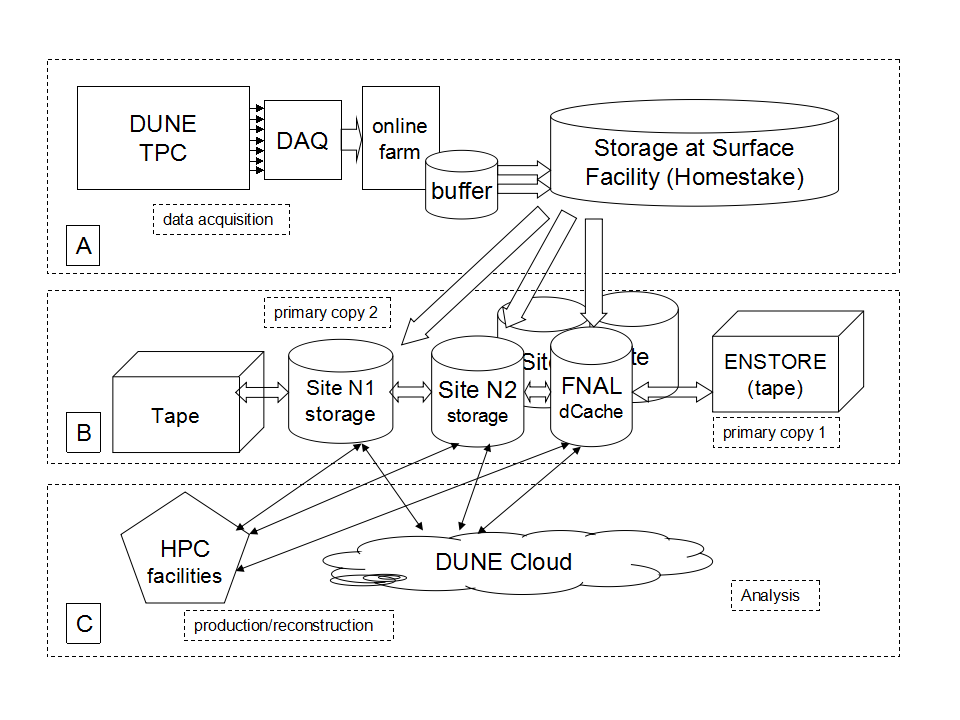
\includegraphics[width=\textwidth]{DUNEdataflow.png}
\caption{Conceptual Diagram of the Data Flow in DUNE.}
\label{fig:DUNEdataflow}
\end{figure}
The top section of the diagram (labeled ``A'') represents systems and data flow at the Far Site.
The mid-section ``B'' depicts the DUNE data storage network. FNAL is the main data center
hosting tape storage for the primary copy of all data, as well as distributed disk (such as dCache).
It is expected that the Metadata system will also be deployed and operated at FNAL.
Additional Grid sites at participating institutions will have replicas of the data.
Replication of the data will be done as per requirements formulated in \ref{sec:req-raw-data-replication}.

\ 
\\

\noindent
\textit{Data Buffering at the Far Site} 
\ 
\\
\noindent
Data Acquisition systems will be located in the specially built rooms in the detector vicinity,
i.e. in the cavern deep underground (commonly referred to as 4850L). The undergound location is to be
connected to surface by 96-strand fiber optic cable, but this does not imply that all strands will be
utilized at any given time. The scale of bandwidth of an individual fiber is 10gbps. It can be therefore
expected that there will be ample headroom for data transmission to the surface under a variety of scenarios.

There will be two layers of data buffering: a buffer in DAQ before the data is transmitted to the surface,
and at the surface facility before the data is transmitted to FNAL which is the primary storage site and the
keeper of the custodial copy of the data.

It is a common practice to provide buffer space for the experiment which is sufficient for intermediate storage of data
for one or maybe a few days in order to keep running even in case of network equipment outages. Given the estimates
presented above, the decisive factor for determining the buffer size will be the data scale of candidate SNB events since
they are likely to be read out at full-stream rate (with lax or no zero-suppression) (see Table~\ref{tab:zs-volume}). The
size of each buffer (the online farm and the surface facility as drawn in section ``A'' of Fig.\ref{fig:DUNEdataflow})
can therefore be estimated as $\sim$50\,TB.
\ 
\\

\noindent
\textit{Data Merging at the Far Site} 
\ 
\\
\noindent
There are additional considerations due to the modular structure of the DUNE Far Detector
which is conceived as four individual TPC modules. In order have to have more flexibility and to minimize down time
and the number of potential single points of failure the DAQ will be segmented into four individual  systems each collecting
data from their respective module~(see \ref{sec:daq-architecture}). To ensure
consistency and simplicity of processing, it is desirable to merge the data streams coming from individual
detectors' DAQ systems at some point so that data is written to files contains readout for the full 4-module
DUNE detector. The surface facility is the optimal location for the merging to take place since it needs to be
equipped with storage and networking equipment for buffering purposes in any scenario.

\ 
\\
\noindent
\textit{SNB vs Other Types of Data} 
\ 
\\
\noindent
According to estimates presented in Table~\ref{tab:summary-data-table} the scale of the SNB candidate date  is vastly larger than
that of beam-$\nu$ and cosmic-$\mu$ events. In addition to size there are other differences -- while data from these other classes of events
can be expected to be coming at a steady (and low) rate, the SNB candidate event will result in large burst of data both in terms of
instantaneous rate and the volume to be collected during the O(1,s) readout window activated by the SNB trigger logic in DAQ.
There are a few reasons to handle the SNB data stream separately from other data.

First, it may be desirable to run a near-time
analysis on portions of the SNB data to determine the veracity of the SNB trigger decision. This can be done at the Far Site surface facility
and is subject to pending R\&D.
%For this to be practical, transmission of the data from 4850L to the surface will need to be done
%at the maximum rate possible.
It is envisioned that in the event of the SNB trigger the DAQ system will put all other logic ``on hold''
in order to ensure full bandwidth and local (DAQ) computing resources are fully dedicated to caputring these data.
%Having multiple strands of optic fiber (as stipulated in current engineering plans) will be crucial to ensure that the data can arrive
%to the surface at almost the same rate as it is produced

Second, having a substantially more modest data stream containing beam neutrino and cosmic ray
events will make processing and distribution of these data to the Collaboration a lot quicker and more efficient.

Finally, there are simply 
no clear benefits of merging the SNB candidates with the rest of the data. It is assumed in this section that it is to be handled
separately e.g. kept in separate datasets.
%The following description applies to the data attributed to beam neutrinos and to the cosmic ray muons.
%Due to the vastly different scale and rate of occurance of the Supernova Burst candidate events, it is not optimal to include this type data in the same
%data stream with $\nu$ and $\mu$.

\ 
\\

\noindent
\textit{Data Transmission from the Far Site} 
\ 
\\
\noindent
Two horizontal arrows in section ``A'' of the diagram in Fig.\ref{fig:DUNEdataflow} represent the WAN connection of
the Far Site to FNAL. Looking at the raw data section of Table~\ref{tab:summary-data-table}, one can estimate
the sustained bandwidth required to transmit all data produced under current set of assumptions as 20\,MB/s (once
again, transmission of buffered SNB candidate data would take most of this bandwidth while items like beam $\nu$
will not occupy an appreciable portion of the bandwidth).

\subsubsection{Data Handling at the Near Site}

The Near Site is located within the boundaries of Fermilab and therefore will have a LAN connection to mass storage
and other central facilities. Raw data will be buffered in the NDS DAQ. Data transmission will be fully automatic and monitored.
Metadata will be managed under the same umbrella as the Far Detector data.

\subsubsection{Interfaces to FNAL Storage Infrastructure}
Both the Far Detector and Near Detector Systems will need to interface storage infrastructure at FNAL.
File catalog and Metadata requriements are listed in~\ref{sec:file-catalog-req}~and~\ref{sec:metadata-req}.
While technology options and choices may be very different at the time of DUNE commissioning from what they
are at the time of writing, it is instructuve to review what exists at Fermilab at present as one possibility of the
configuration to be utilized by DUNE..
Elements of this infrastructure relevant to this dicscussion are:
\begin{itemize}
\item Enstore: tape drive and tape management system.

\item SAM: ``Sequential data Access via Meta-data'', a file based data management and access layer between the Storage Management System
and the data processing layers, developed and maintained at FNAL~\cite{sam_chep12}.

\item dCache: a FNAL instance of a massive distributed storage management system, featuring a virtual filesystem tree with a variety of standard access methods
~\cite{dcache_chep12}

\item BlueArc: Mass Storage, disk-based.

\end{itemize}

\begin{figure}[h!]
\centering
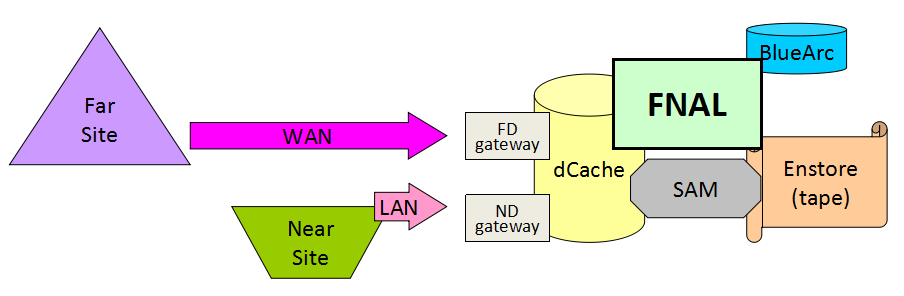
\includegraphics[width=0.8\textwidth]{fnal-data-infrastructure-sketch-1.png}
\caption{Conceptual Diagram of FD and NF interface to storage infrastructure at FNAL.}
\label{fig:fnal-data-infrastructure}
\end{figure}

\noindent
A key part of interaction of the DUNE data transport system and storage infrastructure at FNAL is generation and management of
Metadata. In the illustration given in Fig.~\ref{fig:fnal-data-infrastructure} this functionality resides in ``SAM'' (or its future equivalent).
When a unit of data arrives and is deposited in the designated ``dropbox'' to be picked up by SAM services for placement into mass storage,
appropriate metadata is generated according to prepared specifications and added to SAM database.

An important feature of dCache storage at FNAL is that it is available to the outside world via the so-called ``xrootd door''. Having a standard
access method to substantial amount of storage located at FNAL allows for creation of powerful tools for sharing and distribution of data in DUNE.

\subsubsection{Raw Data Replication and Retention}
Requirements for raw data replication are listed in~\ref{sec:req-raw-data-replication}. Sites with appropriate characteristics
(e.g. storage capacity, network access bandwidth etc) shall be selected for purpose of raw data replication before DUNE
commissioning and to allow sufficient time for integration testing.
Raw data for both Far and Near Detector Subsystems will be replicated. There will be no less than one full copy of raw
data and likely two. A replica does not need to reside at a single data center in its entirety, i.e. replicas will be allowed to span
more than one data center. To be effective replication must rely on proper management of Metadata, so it makes sense
for FNAL to be the center of worldwide data replication in DUNE.

Policies regarding retention of raw data shall be set in accordance with \ref{sec:req-raw-data-retention}.

\subsection{Production}
\subsubsection{Production Streams}
Three distinct production streams can be identified in DUNE:
\begin{itemize}
\item Far Detector beam-$\nu$, cosmic-$\mu$ and nucleon decay candidate events (all in shared datasets)

\item Far Detector Supernova Burst candidate events (in separate datasets)

\item Near Detector Systems data (in separate datasets)
\end{itemize}

\subsubsection{First-pass Production (Far Detector Data)}

First-pass
%ESD
production will take place at FNAL after the data is received and catalogued in SAM.
As mentioned above, SNB candidate data will be handled separately (reside in datasets separate from
other types of data) and for this reason will require dedicated production runs.

The low rate of the beam-$\nu$ and cosmic-$\mu$ triggers (see Table \ref{tab:zs-volume}) allows for
prompt first-pass reconstruction to be handled at FNAL as soon as these data are received, using the
``best available'' calibration data. At the time of writing
a number of reconstruction techniques are being considered for use in DUNE (see Appendix~\ref{sec:reconstruction})
and the range of CPU requirements
for this production step is still fairly wide, however given that the number of cosmic-$\mu$ candidates will be roughly $\sim$10$^3$ per hour
it can be expected that Fermigrid should be able to provide the necessary resources. Assuming 
that it would take O(10\,min) of CPU time on a typical worker node to reconstruct an event of medium complexity
(as is the case with a few software tools currently in use),
a farm of 1,000 worker nodes will be capable of processing data at same rate as it is received.

Data structures and formats such as ESD and AOD-types are still in development at the time of writing so no separate
description of these in the production chain can be produced.

\subsubsection{Calibrations and Reprocessing (Far Detector Data)}
Calibration procedures are briefly described in~\ref{sec:daq-calibrations}. Since cosmic muon events present in the data
are a crucial element for cross-checks and verifying the energy scale for TPC measurements, calibrations will depend on
the first-pass production in what is essentially an iterative process.

Once a set of  refined calibration data is produced, reprocessing will take place at FNAL and other participating institutions.
Aside from reprocessing runs producing more precise data due to better calibrations, it will be necessary to repeat processing
for different reasons, such as introduction of new software releases, their testing and validation etc.
As stated in comments to Table~\ref{tab:summary-data-table} on page~\pageref{tab:summary-data-table}, the storage requirements estimations in this table include
a ``headroom factor'' of 4 to effectively account for storage necessary for reprocessing.

\subsubsection{Production for the Near Detector Systems Data}
The Near Detector Systems in DUNE feature considerable complexity of design and operations, and set ambitious goals
for precision measurement of both momenta (via tracking in the magnetic field) and energy (via calororimetry). This leads to
potentially complex calibrations. While based on same general principles as production for the Far Detector, the NDS processing
will be done in separate production streams. While not much detail is known about the eventual choice of data formats and algorithms for
the NDS, it is reasonable to assume that same approach (first-pass at the data and then reprocessing based on refined calibration)
will be used as for the Far Detector.


\subsection{DUNE Analysis}
\subsubsection{Analysis Procedures and Data Flow}
As mentioned above, the SNB candidate data stands apart from other sources of data and will be assigned
a separate processing and analysis chain. Assuming the nominal rate
of false positives of 12 per year, it is estmated that roughly 50\,TB of SNB candidate data will need to be processed
monthly (see Table~\ref{tab:zs-volume}). Once an analysis pass is done with a candidate event, it can be expected
that the event can be committed to permanent storage on tape.

The Far Detector datasets outside of the SNB category will be dominated by cosmic muon events and nucleon decay candidates.
As indicated in Table~\ref{tab:summary-data-table}, the associated data volume is modest and of the order of 40\,TB annually.
On this scale the data can be shipped to member institutions using a variety of methods for analysis (see~\ref{sec:data-mgt}).

Handling the Near Detector data will be somewhat more challenging to a larger projected volume: $\sim$100\,TB of raw data annualy
as per Table~\ref{tab:summary-data-table}, and some eight times more than that if one models the storage requirements for NDS on
same basis as for the Far Detector (extrapolation of the derived data volume plus the ``headroom factor'' for reprocessing).

\subsubsection{Distribution of Analysis Workload}
In order to leverage the intellectual resources of the Collaboration, it will be necessary to implement easy and ready access to
requisite data analysis facilities to members of DUNE. It can be expected that researchers will use different modes of analyzing
the data depending on the stage of analysis -- for example significantly reduced datasets containing Derived Physics Data
may be compact enough to be used efficiently on users' workstations and laptops. Earlier stages of data derivations
involve larger amounts of data and it may become necessary to provide distributed analysis facilities similar to what the LHC
experiments have deployed, via their respective Workload Management Systems (\ref{sec:dune-wms}).

\subsection{Simulation}
Producing simulated data is the type of workload that can be handled efficiently by data centers at DUNE member institutions
since it puts less stringent requirements on the bandwidth available to the site.
Such data must be made avaialbe for all of Collaboration. Estimates of the MC data and data derived from it are also given
in Table~\ref{tab:summary-data-table}.

%\subsubsection{The Analysis Model}
%\subsubsection{Distributed Analysis}

\subsection{Data Management}
\label{sec:data-mgt}
\subsubsection{LHC Experience with Data Distribution}
\label{sec:data-monarc}
In formulating the architecture for data distribution in DUNE, it is helpful to study the experience of the LHC experiments,
since DUNE shares much of the same challenges: potentially significant  volume of data to be collected and processed,
projected long period of operation of the experiment, and geographically dispersed and diverse research communities joining the Collaboration.

When data management systems for the LHC experiments were designed and deployed around the turn of the century, it had to be done
against the backdrop of lack of universal access to high bandwidth networks across collaborations and/or substantial cost of such access~\cite{monarc},
along with reliability issues.
In order to maximize utilization of intellectual and technical resources spread around the globe, a model was adopted in which the computing resources
were organized as a hierarchy of Regional Centers, which allowed for tight control and optimization of data transmission. In this hierarchy, the following
levels were identified:
\begin{itemize}
\item Tier-0: CERN
\item Tier-1: National Center (``large scale and expensive facility'')
\item Tier-2: Regional Center (``smaller, mostly for analysis, local center of expertise and maintenance'')
\item Tier-3: Workgroup Servers at participating institutions
\item Tier-4: Individual computers (desktops)
\end{itemize}
\noindent
In this approach, distribution of data and access to it within an experiment is likewise hierarchical, as shown in Fig.\ref{fig:monarc}.
\begin{figure}[h!]
\centering
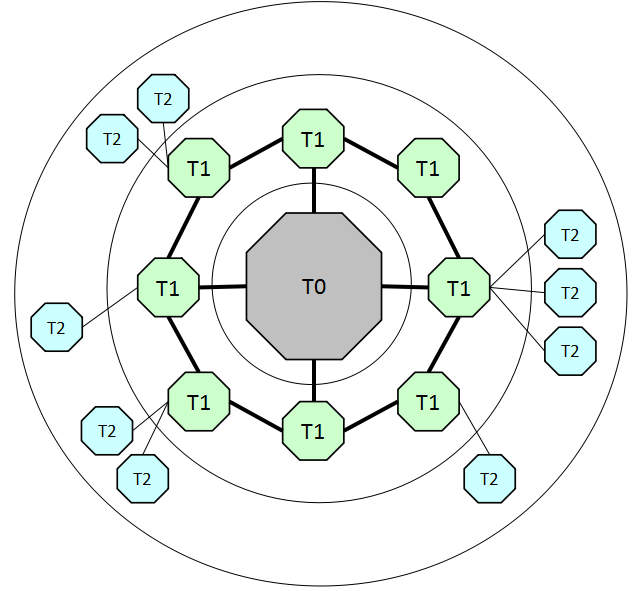
\includegraphics[width=0.6\textwidth]{monarc-model.png}
\caption{MONARC model of data distribution.}
\label{fig:monarc}
\end{figure}
Tier-1 centers have assured high bandwidth to CERN (Tier-0) which is typically achieved by establishing a dedicated
optical fiber connection with properly equipped endpoints. Tier-1 facilities form the the basis of further distribution of data
as required, in particular serving data to Tier-2.

Tier-2 centers would not be typically engaged in large scale production activities involving raw data and thus
have reduced network requirements. Smaller Tier-3 facilities would access data via Tier-2 etc.

We observe that at present, these experiments have actually revised the approaches to Data Handling and Workload
Management adopted in preparation for LHC Run-1~\cite{lhc_model_update}.
\begin{figure}[h!]
\centering
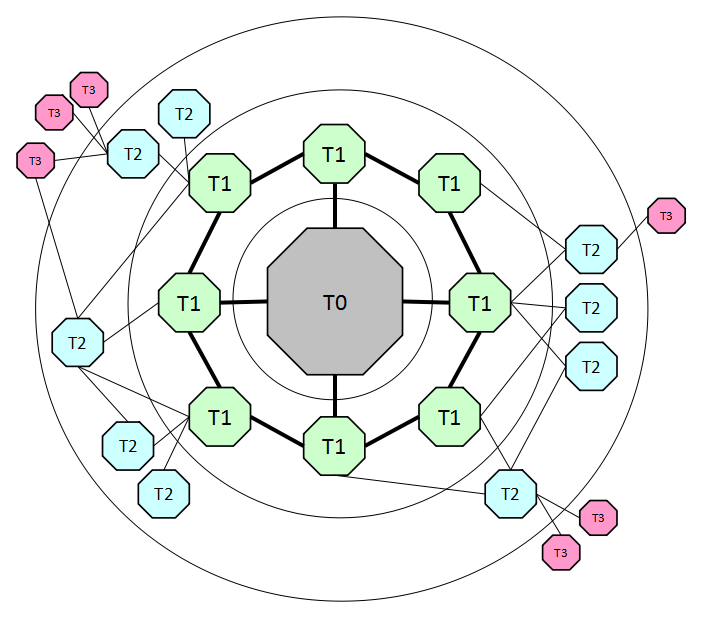
\includegraphics[width=0.6\textwidth]{un-monarc-model.png}
\caption{Evolved LHC model of data distribution.}
\label{fig:un-monarc}
\end{figure}
For Data Handling, there is a marked transition from the strictly hierarchical
“tiered” model of data distribution and access (e.g. MONARC) to more flat, agile, scalable and more peer-to-peer-like
architectures (see Fig.~\ref{fig:un-monarc}).
As stated in~\cite{lhc_model_update}
\begin{quotation}
\textit{With the technological progress of wide area networks and consequently improved network connectivity ATLAS has
already in Run-1 gradually moved away from the hierarchical association of Tier-2s to one Tier-1 (MONARC model)
and is now able to associate workflows between a well-connected Tier-2 and several Tier-1s, based on monitored
connectivity metrics. This functionality will be further pursued in Run-2 and is being incorporated into the production
system and distributed data management developments.}
\end{quotation}

\noindent
For Workload Management, the LHC computing models have evolved to put emphasis on access to heterogeneous and sometimes
opportunistic resources, facilitated by dynamic software provisioning. Other challenges being addressed in LHC computing include
the design and handling of Metadata, and managing computational workflows.


\subsubsection{Distributed Data Management}
For its Distributed Data Management, DUNE will use the experience gained by the LHC experiments (\ref{sec:data-monarc}) and will
take the same direction of its evolution. In practice this means the ``data in the network'' approach adopted by ATLAS in the form of its FAX system,
and the AAA system created by CMS.


\subsubsection{Databases}
Requirements for DUNE Databases have been described in \ref{sec:req-db}.


\subsection{Workload Management}
\label{sec:dune-wms}
For DUNE requirements to its Workload Management System please see \ref{sec:req-wms}. There are a few systems currently used by various experiments which
differ in the following aspects:
\begin{itemize}

\item Degree of integration with their corresponding data management system.

\item Depth and breadth of monitoring capabilities offered by the system to the user and to the expeiment's operations team.

\item Ability to handle complex workflows automatically.

\item Functionality to correct various error conditions and failure modes, for example ``retry'' a set of jobs that were stuck in an unfinished state
due to corrupted or otherwise missing data and other such conditions.

\end{itemize}

\noindent
A few examples of widely deployed WMS include:
\begin{itemize}

\item Dirac (Distributed Infrastructure with Remote Agent Control) WMS~\cite{dirac_wms} used at CERN by LHCb.

\item PanDA (``Production and Distributed Analysis'') \cite{panda_chep13}, which forms the backbone of ATLAS processing and has been used in other experiments such as AMS.
PanDA has scaled up to manage O(10$^6$) Grid jobs daily, upgraded to use a fine-grained workflow management system, added an event service to
make it easier to use short-term opportunistics resource and a host of other features. A distinguishing feature of PanDA is sophisticated and powerful
monitoring system which allows efficient troubleshooting and optimal degree of control over execution of workflows.

\item GlideinWMS \cite{glideinwms_chep13} used in CMS and a variety of projects in other disciplines via the Open Science Grid Consortium.

\item Alien \cite{alien} deployed for the Alice experiment at the LHC.

\end{itemize}

\noindent
FNAL has successfully deployed a Grid toolkit named \textit{jobsub} \cite{jobsub_chep13}, which has been used for a number of years to facilitate users' access to
Grid facilities at FNAL and at other grid sites, such as those participating in the Open Science Grid Consortium \cite{osg}. It integrates FNAL-local access via
HTCondor facilities with GlideinWMS extensions to reach available resources elsewhere.

Where needed, \textit{jobsub} leverages the CVMFS network file system for software provisioning and the \textit{ifdh} data handling tool which integrates
with SAM, dCache, Amason S3 etc.

\subsection{Offline Software}
\subsubsection{Overview}

For s detailed presentation of requirements to DUNE offline software please see Section~\ref{sec:req-software}.
A few important items which will be pursued in DUNE are achitectural compliance, code review, revision control, release methodology,
 and documentation. Due to the large size of the Collaboration and diversity of its distributed
 computing resources DUNE will have to create a ``supported platform'' policy which will define the mechanisms by
which platforms are selected for support, retired from
supported status and what level of support and methods for its delivery will be provided.

Just like the vast majority of other physics experiments in HEP and Intensity Frontier, DUNE relies on the ROOT\cite{root}
system as the foundation of a wide spectrum of its software. It forms the basis for the \textit{art} framework\cite{art},
\textit{artdaq} -- a DAQ framework which is an extension of \textit{art},
and LArSoft -- a software suite for simulation and reconstruction of
events in Liquid Argon TPC, which also also built on top of \textit{art}.

GEANT 4~\cite{geant4} is used in a variety of application in DUNE as the main simulation engine, and it integrated
into LArSoft and other simulation tools. MARS is used for estimation of complex radiological backgrounds and for
beam line simulation.

\subsubsection{Release managememt and Continuous Integration}
At the time of writing DUNE is already investing effort in managing releases of the LArSoft software.
Continuous Integration (CI) services are provided
by FNAL's Scientific Computing Division, and in particular Jenkins \cite{jenkins} system is utilized for CI.

One of the challenges in managing DUNE software is active use of LArSoft across a few experiments in the
Intensity Frontier, which constantly leads to new requirements, features and otherwise results in updates
of the design and interfaces of this software suite. Different branches may have compatibility issues.

\subsubsection{Software provisioning}
DUNE (like its predecessor LBNE) is using a few different methods to deploy its software on sites outside of FNAL,
both for interactive use by delvelopers and researchers and to provision software to  Worker Nodes
in batch system configuration. Currently products like \textit{art} and LArSoft can be built from source (including
the components they depend on, e.g. ROOT) using utilities created and maintained by the FNAL Scientific Computing
Division. This method can be used to make this software available on a cluster or interactive workstations outside
of FNAL.

DUNE is following the common trend of delivering software via the networks, in particular experience has been gained with
CernVM-FS (Cern-VM File System, commonly called CVMFS) \cite{cvmfs}. It is a network file system based on HTTP and
optimized to deliver experiment software in a fast, scalable,
and reliable way. It was originally designed to decouple the life cycle management of the application software releases
from the operating system of a specific configuration of a Virtual Machine, ``CERNVM''. Now it is often used independently
from its original purpose and has proven itself as efficient tool for software delivery to worker nodes in systems and locations
where complete installation (``build'') of DUNE software is not practical or desirable.

